%instiki:category: FisicaSubatomica
\chapter{Modelo Est\'andar}
\label{cha:modelo-estandar} %noinstiki
%instiki:
%instiki:***
%instiki:
%instiki:[[NotasFS|Tabla de Contenidos]]
%instiki:
%instiki:***
%instiki:
%instiki:* [Interacci\'on Electrod\'ebil](#inter-electr)
%instiki:
%instiki:* [Modelo Est\'andar](#modelo-estandar)
%instiki:
%instiki:***
%instiki:

\section{Interacci\'on Electrod\'ebil para leptones}
\label{sec:inter-electr}
El Lagrangiano de Dirac para la primera generaci\'on de leptones representados por los campos $\psi_e$ y $\psi_\nu$, es
\begin{align}
\mathcal{L}=i\overline{e_L}i\gamma^\mu\partial_\mu e_L+i\overline{e_R}i\gamma^\mu\partial_\mu e_R
  +i\overline{\nu_L}\gamma^\mu\partial_\mu\nu_L+i\overline{\nu_R}\gamma^\mu\partial_\mu\nu_R\nonumber\\
  -m_e(\overline{e_L}e_R+\overline{e_R}e_L)
  -m_\nu(\overline{\nu_L}\nu_R+\overline{\nu_R}\nu_L)
\end{align}
donde
\begin{equation}
  \psi_e\equiv e=e_L+e_R,\qquad \psi_\nu\equiv\nu_e=\nu_L+\nu_R\,.
\end{equation}
Este Lagrangiano debe dar cuenta de las caracter\'\i sticas de las interacciones d\'ebiles.
\subsection*{Corrientes V--A}
\label{sec:corrientes-v}
En dichas interacciones s\'olo participan las partes izquierdas de los campos. Esto nos permite prescindir del $\nu_R$, pues no tiene cargas d\'ebiles, fuertes o el\'ectricas
\begin{align}
  \label{eq:261}
  \mathcal{L}=i\overline{e_L}\gamma^\mu\partial_\mu e_L+i\overline{e_R}\gamma^\mu\partial_\mu e_R
  +i\overline{\nu_L}i\gamma^\mu\partial_\mu\nu_L-m_e(\overline{e_L}e_R+\overline{e_R}e_L)
\end{align}

\subsection*{Simetr\'\i a global $SU(2)_L\times U(1)_Y$}
\label{sec:simetr-glob-su2_l}

En el contexto de las interacciones d\'ebiles un $e_L$ es completamente equivalente a un campo $\nu_L$. Es decir, el Lagrangiano debe ser invariante bajo una transformaci\'on $SU(2)_L$ de esos campos. La diferencia entre ellos son sus respectivas cargas electricas y sus masas. Asumiendo que ambos campos tienen la misma hipercarga, podr\'\i amos esperar que la corriente electromagn\'etica apropiada puede obtenerse a partir del Grupo semisimple $SU(2)_L\times U(1)_Y$. Adem\'as las respectivas masas se podr\'\i an obtener a partir del mecanismo de Higgs. De hecho, definiendo el doblete 
  \begin{align}
    L\equiv\begin{pmatrix}
      \nu_L\\
      e_L      
    \end{pmatrix}\,,
  \end{align}
este transforma bajo $SU(2)_L$ como
\begin{align}
  L\to L'=&\exp(i T^i \theta_i)L\approx(1+i T^i\theta_i)L\nonumber\\
  \begin{pmatrix}
    \nu'_L\\
    e'_L
  \end{pmatrix}\approx&\begin{pmatrix}
    1+\frac{i}{2}&\frac{i}{2}\sqrt{2}\left(\frac{\theta_1-i\theta_2}{\sqrt{2}}\right)\\
    \frac{i}{2}\sqrt{2}\left(\frac{\theta_1+i\theta_2}{\sqrt{2}}\right)&1-i\frac{1}{2}
  \end{pmatrix}\begin{pmatrix}
    \nu_L\\
    e_L
  \end{pmatrix}\nonumber\\
  =&\begin{pmatrix}
    1+\frac{i}{2}&\frac{i}{2}\sqrt{2}\,\theta^+\\
    \frac{i}{2}\sqrt{2}\,\theta^-&1-i\frac{1}{2}
  \end{pmatrix}\begin{pmatrix}
    \nu_L\\
    e_L
  \end{pmatrix}\nonumber\\
  =&\begin{pmatrix}
    \left(1+\frac{i}{2}\right)\nu_L+\frac{i}{2}\sqrt{2}\,\theta^+e_L\\
    \left(1-\frac{i}{2}\right)e_L+\frac{i}{2}\sqrt{2}\,\theta^-\nu_L\\
  \end{pmatrix}\,.
\end{align}
Claramente el t\'ermino de masa $m_e$ en la ec.~(\ref{eq:261}) no es invariante bajo esta transformaci\'on. El Lagrangiano en la ec.~(\ref{eq:261}), sin t\'ermino de masa, puede reescribirse de manera que exhiba de forma m\'as explicita la invariante bajo $SU(2)_L$ como
\begin{align}
  \label{eq:219}
 \mathcal{L}=i\overline{L}\gamma^\mu\partial_\mu L+i\,\overline{e_R}\gamma^\mu\partial_\mu e_R\,,
\end{align}
donde, bajo $SU(2)_L$ $e_R$ transforma como
\begin{align}
  e_R\to e'_R=e_R\,.
\end{align}
Para que el Lagrangiano en la ec.~(\ref{eq:219}) sea invariante gauge global bajo $SU(2)_L\times U(1)_Y$, se debe satisfacer la relaci\'on de Gell--man--Nishijima \eqref{eq:184}
\begin{align}
  Q L=&
  \begin{pmatrix}
    0 \nu_L\\
    -1 e_L 
  \end{pmatrix}=
 (T_3+Y) L=
 \begin{pmatrix}
   \left(\frac{1}{2}+Y_L\right)\nu_L\\
   \left(-\frac{1}{2}+Y_L\right)e_L
 \end{pmatrix}
\nonumber\\
  Q e_R =&-1 e_R= Y\, e_R =Y_R\, e_R\,,
\end{align}
de modo que
\begin{align}
  Y_L&=-\frac{1}{2}& Y_R&=-1\,.
\end{align}
Concluimos que para que la simetr\'\i a gauge local bajo $SU(2)_L\times U(1)_Y$ sea exacta se requiere que la hipercarga $Y$ de ambas componentes del doblete sea la misma y que ambas tengan masa cero. Para tener un modelo consistente debe existir un mecanismo para generar la masa del electr\'on. 
\subsection*{Simetr\'\i a local $SU(2)_L\times U(1)_Y$}
\label{sec:simetr-local-su2_l}
Para que las cargas de isosp\'\i n d\'ebil se conserven localmente debemos cambiar la derivada normal en el Lagrangiano \eqref{eq:219} por la derivada covariante de $SU(2)_L\times U(1)_Y$
\begin{align}
  \label{eq:125}
  \partial^\mu\to\mathcal{D}^\mu&\equiv\partial^\mu-igT^iW^\mu_i-ig'YB^\mu\nonumber\\
&=  \begin{pmatrix}
    \partial^\mu-igT_3^\uparrow W^3_\mu-ig'YB_\mu&\frac{1}{\sqrt{2}}gW^+_\mu\\
    \frac{1}{\sqrt{2}}gW^-_\mu&\partial^\mu+igT_3^\downarrow W^3_\mu-ig'YB_\mu
  \end{pmatrix}.
\end{align}
y el Lagrangiano
\begin{align}
  \label{eq:220}
   \mathcal{L}=i\overline{L}\gamma^\mu\mathcal{D}_\mu L+i\,\overline{e_R}\gamma^\mu\mathcal{D}_\mu e_R
-\tfrac{1}{4}W^{\mu\nu}_i W_{\mu\nu}^i-\tfrac{1}{4}B^{\mu\nu} B_{\mu\nu}\,,
\end{align}
es el Lagrangiano invariante gauge local m\'as general posibles para los campos $e_{L,R}$, $\nu_L$, $W^\mu_i$, y $B^\mu$. De acuerdo a la ec.~\eqref{eq:124}
\begin{align}
  W^{\mu\nu}_i=\partial^\mu W^\nu_i -\partial^\nu W^\nu_i+g\,\epsilon^{ijk}W^\mu_j W^\nu_k.
\end{align}
Para escribir el Lagrangiano en una forma compacta, debemos introducir una convenci\'on: siempre que los t\'erminos de $\mathcal{D}^\mu$ act\'uen en un estado fermi\'onico de forma matricial diferente, el resultado es cero por definici\'on. As\'\i{} el resultado de hacer actuar $T^iW^\mu_i$ sobre el singlete bajo $SU(2)_L$, $e_R$, es cero. Note que
\begin{align}
  \mathcal{D}_\mu e_R=(\partial_\mu-ig' Y_R B_\mu)e_R\,.
\end{align}
En la secci\'on \ref{sec:invar-gauge-local-1} vimos que para tratar consistentemente el electromagnetismo conjuntamente con el grupo gauge local $SU(2)$, era necesario suponer inicialmente la existencia de un bos\'on gauge $B^\mu$ asociado a un grupo $U(1)_Y$ en lugar del $A^\mu$ electromagn\'etico asociado a $U(1)_Q$. El $A^\mu$ se puede obtener posteriormente a partir de una combinaci\'on lineal apropiada de $B^\mu$ y $W^\mu_3$, el bos\'on gauge diagonal de $SU(2)$. 

\subsection*{Mecanismo de Higgs}
\label{sec:mecanismo-de-higgs-1}
Como los bosones gauge $W^\mu_i$ deben ser masivos para dar cuenta de que la interacci\'on d\'ebil es de corto alcance, el Lagrangiano en ec.~\eqref{eq:220} debe ser complementado con un potencial escalar apropiado que pueda dar lugar a una ruptura espont\'anea de la simetr\'\i a. De acuerdo a la discusi\'on del Cap\'\i tulo \ref{rupt-espont-de} la escogencia m\'\i nima es introducir un doblete escalar complejo
\begin{equation}
  \Phi=
  \begin{pmatrix}
    \phi^+\\
    \phi^0
  \end{pmatrix}\,.
\end{equation} 
Entonces
\begin{align}
  \label{eq:221}
     \mathcal{L}=i\overline{L}\gamma^\mu\mathcal{D}_\mu L+i\,\overline{e_R}\gamma^\mu\mathcal{D}_\mu e_R
     -\tfrac{1}{4}W^{\mu\nu}_i W_{\mu\nu}^i-\tfrac{1}{4}B^{\mu\nu} B_{\mu\nu}
+(\mathcal{D}_\mu\Phi)^\dagger\mathcal{D}^\mu\Phi-\mu^2\Phi^\dagger\Phi-\lambda(\Phi^\dagger\Phi)^2\,,
\end{align}
donde $\mu^2\lt 0$, y $\lambda\gt 0$.



Los t\'erminos bos\'onicos en la ec.~(\ref{eq:221}), ya fueran analizados en la secci\'on \ref{sec:mecanismo-de-higgs},  eq.\eqref{eq:97}. 

\subsection*{Lagrangiano de Yukawa}
Para los campos del Lagrangiano en eq.~(\ref{eq:221}), debemos asegurarnos de que todos los t\'erminos invariantes gauge locales y renormalizables sean considerados. De hecho un t\'ermino de interacci\'on entre fermiones y el campo escalar, correspondiente a una interacci\'on de Yukawa, resulta ser invariante gauge local. Incluyendo dicho t\'ermino en el Lagrangiano invariante $SU(2)_L\times U(1)_Y$ para los campos $e$, $\nu_L$, $W_\mu^i$, $B_\mu$ y $\Phi$ tenemos
\begin{align}
  \label{eq:226}
     \mathcal{L}=&i\overline{L}\gamma^\mu\mathcal{D}_\mu L+i\,\overline{e_R}\gamma^\mu\mathcal{D}_\mu e_R\nonumber\\
     &-h_e\overline{L}\Phi e_R-h_e\overline{e_R}\Phi^\dagger L\nonumber\\
     &-\tfrac{1}{4}W^{\mu\nu}_i W_{\mu\nu}^i-\tfrac{1}{4}B^{\mu\nu} B_{\mu\nu}\nonumber\\
     &+(\mathcal{D}_\mu\Phi)^\dagger\mathcal{D}^\mu\Phi-\mu^2\Phi^\dagger\Phi+\lambda(\Phi^\dagger\Phi)^2\,.
\end{align}
Bajo una transformaci\'on gauge local los campos transforman como:
\begin{align}
  \mathcal{D}_\mu L&\to\left(\mathcal{D}_\mu L\right)'=\exp\left(-iT^i\theta_i-iY_L\right)\mathcal{D}_\mu L\nonumber\\
  \mathcal{D}_\mu e_R&\to\left(\mathcal{D}_\mu e_R\right)'=\exp\left(-iY_R\right)\mathcal{D}_\mu e_R\nonumber\\
  \Phi&\to\Phi'=\exp\left(-iT^i\theta_i-iY_\Phi\right)\Phi,
\end{align}
Y la acci\'on determinada por el Lagrangiano en ec.~\eqref{eq:226} permanece invariante bajo $SU(2)_L\times U(1)_Y$. Parte de los t\'erminos del Lagrangiano ya han sido analizados en el Cap\'\i tulo \ref{rupt-espont-de}. 

\subsection*{Gauge Unitario}
Para obtener el espectro despu\'es de la ruptura espont\'anea de simetr\'\i a es conveniente usar el Gauge Unitario para reescribir el campo de Higgs como en la ec.~\eqref{eq:123}
\begin{equation}
      \Phi=
  \begin{pmatrix}
    0\\
    \frac{1}{\sqrt{2}}[H(x)+v]
  \end{pmatrix}\,.
\end{equation}
Usando los resultados de la secci\'on \ref{sec:mecanismo-de-higgs} tenemos
\begin{align}
  \mathcal{L}_{H W B}=&\left(\mathcal{D}^\mu\Phi\right)^\dagger\mathcal{D}_\mu\Phi-\mu^2\Phi^\dagger \Phi-\lambda\left(\Phi^\dagger\Phi\right)^2\nonumber\\
  =&\frac{1}{2}\partial^\mu H\partial_\mu H-V(H)\nonumber\\
&+\frac{1}{4}g^2{W^\mu}^-W_\mu^+H^2+\frac{1}{2}vg^2{W^\mu}^-W_\mu^+H\nonumber\\
  &+\frac{1}{2}\left(\frac{g}{2\cos\theta_W}\right)^2Z^\mu Z_\mu H^2+\left(\frac{g}{2\cos\theta_W}\right)^2v\,Z^\mu Z_\mu H\nonumber\\
  &+\frac{1}{2}m_W^2{W^\mu}^-W_\mu^++\frac{1}{2}m_W^2{W^\mu}^-W_\mu^+ +\frac{1}{2}m_Z^2Z^\mu Z_\mu\,,
\end{align}
donde:
%instiki:
\begin{itemize} %noinstiki
\item
  \begin{align}
    V(H)=&\tfrac{1}{2}m_H^2H^2+\lambda vH^3+\tfrac{1}{4}\lambda H^4\nonumber\\
    =&\frac{1}{2}m_H^2H^2+\frac{m_H^2}{2v}H^3+\frac{1}{4}\frac{m_H^2}{2v^2} H^4\nonumber\\
    =&\frac{1}{2}m_H^2H^2\left(1+\frac{H}{v}+\frac{H^2}{4v^2}\right)\,.
  \end{align}
con
\begin{equation}
  m_H^2=-2\mu^2=2\lambda v^2.
\end{equation}

\item 
\begin{equation}
\label{eq:262}
  \begin{pmatrix}
    W^3_\mu\\
    B_\mu
  \end{pmatrix}=\begin{pmatrix}
    \cos\theta_W & \sin\theta_W\\
    -\sin\theta_W& \cos\theta_W
  \end{pmatrix}
  \begin{pmatrix}
    Z_\mu\\
    A_\mu
  \end{pmatrix},
\end{equation}
tal que
\begin{equation}
  \label{eq:263}
  g\sin\theta_W=g'\cos\theta_W=e.
\end{equation}
\item
  \begin{equation}
    m_W=\frac{gv}{2}\qquad m_Z=\frac{m_W}{\cos\theta_W}.
  \end{equation}
\end{itemize} %noinstiki
%instiki:
Entonces
\begin{align}
\mathcal{L}_{H W B}=&\frac{1}{2}\partial^\mu H\partial_\mu H-V(H)\nonumber\\
&+m_W^2{W^\mu}^-W_\mu^++\frac{g^2v^2}{4v^2}(2vH+H^2){W^\mu}^-W_\mu^+\nonumber\\
  &+\frac{1}{2}m_Z^2Z^\mu Z_\mu+\frac{1}{2v^2}\left(\frac{gv}{2\cos\theta_W}\right)^2(2vH+H^2)Z^\mu Z_\mu\nonumber\\
  =&\frac{1}{2}\partial^\mu H\partial_\mu H-V(H)
  +m_W^2\left(1+2\frac{H}{v}+\frac{H^2}{v^2}\right){W^\mu}^-W_\mu^+
  +\frac{1}{2}m_Z^2\left(1+2\frac{H}{v}+\frac{H^2}{v^2}\right)Z^\mu Z_\mu\,.
\end{align}
Adem\'as
\begin{align}
  \mathcal{L}_{l W B}=&i\overline{L}\gamma^\mu\mathcal{D}_\mu L+i\,\overline{e_R}\gamma^\mu\mathcal{D}_\mu e_R
\end{align}
Donde, usando el mismo procedimiento se obtiene el resultado an\'alogo para la ec.~\eqref{eq:187}
\begin{align}
 \mathcal{L}_{l W B}=i\overline{L}\gamma^\mu[\partial_\mu-i g (T^1W_\mu^1+T^2W_\mu^2)-i(g T^3W_\mu^3+g' Y B_\mu)]L
+i\overline{e_R}\gamma^\mu(\partial_\mu-i g' Y B_\mu)e_R
\end{align}
Ya que
\begin{align}
  T^1W_\mu^1+T^2W_\mu^2=&\frac{1}{2}
  \begin{pmatrix}
    0             &W_\mu^1-i W_\mu^2\\
    W_\mu^1-i W_\mu^2  & 0          \\
  \end{pmatrix}=\frac{\sqrt{2}}{2}
  \begin{pmatrix}
    0             &W_\mu^+\\
    W_\mu^-  & 0          \\
  \end{pmatrix}
\end{align}
\begin{align}
\mathcal{L}_{l W B}=&i\overline{\nu_L}\gamma^\mu\partial_\mu\nu_L+i\overline{e_L}\gamma^\mu\partial_\mu e_L
+i\overline{e_R}\gamma^\mu\partial_\mu e_R+
  \frac{g}{\sqrt{2}}\begin{pmatrix}
    \overline{\nu_L}&\overline{e_L}
  \end{pmatrix} 
  \begin{pmatrix}
    0             &W_\mu^+\\
    W_\mu^-  & 0          \\
  \end{pmatrix}
  \begin{pmatrix}
    \nu_L\\
    e_L
  \end{pmatrix}\nonumber\\
&+\overline{L}\gamma^\mu\left(\frac{g}{2}\tau_3W_\mu^3+g'Y B_\mu\right)L+
g'\overline{e_R}\gamma^\mu Y_R B_\mu e_R
\end{align}
usando ec.~\eqref{eq:262}
\begin{align}
  \mathcal{L}_{l W B}=&i\overline{\nu_L}\gamma^\mu\partial_\mu\nu_L+i\overline{e}\gamma^\mu\partial_\mu e
+\frac{g}{\sqrt{2}}\left(\overline{e_L}W_\mu^-\nu_L+\overline{\nu_L}W_\mu^+e_L\right)+\nonumber\\
&\overline{L}\gamma^\mu\left[\frac{g}{2}\tau_3(c_W Z_\mu+s_W A_\mu)
+g'Y(-s_W Z_\mu+c_W A_\mu)\right]L+\nonumber\\
&g'\overline{e_R}\gamma^\mu Y_R(-s_W Z_\mu+c_W A_\mu) e_R\nonumber\\
=&i\overline{\nu_L}\gamma^\mu\partial_\mu\nu_L+i\overline{e}\gamma^\mu\partial_\mu e
+\frac{g}{\sqrt{2}}\left(\overline{e_L}W_\mu^-\nu_L+\overline{\nu_L}W_\mu^+e_L\right)+\nonumber\\
&\overline{L}\gamma^\mu\left[\left(\frac{g c_W}{2}\tau_3 -g's_W Y \right)Z_\mu
+\left(\frac{g s_W}{2}\tau_3 +g'c_W Y \right)A_\mu\right]L\nonumber\\
&-g's_W\overline{e_R}\gamma^\mu Y_R Z_\mu e_R+g'c_W\overline{e_R}\gamma^\mu Y_R A_\mu e_R
\end{align}
usando ec.~(\ref{eq:263})

\begin{align}
\mathcal{L}_{l W B}=&i\overline{\nu_L}\gamma^\mu\partial_\mu\nu_L+i\overline{e}\gamma^\mu\partial_\mu e
+\frac{g}{\sqrt{2}}\left(\overline{e_L}W_\mu^-\nu_L+\overline{\nu_L}W_\mu^+e_L\right)+\nonumber\\
&\overline{L}\gamma^\mu\left(\frac{g c_W}{2}\tau_3 -g\frac{s^2_W}{c_W} Y \right)L Z_\mu
+e\overline{L}\gamma^\mu\left(\frac{\tau_3}{2} + Y \right) L A_\mu\nonumber\\
&-g \frac{s^2_W}{c_W}\overline{e_R}Y_R e_R Z_\mu+e \overline{e_R}Y_R e_R A_\mu\nonumber\\
=&i\overline{\nu_L}\gamma^\mu\partial_\mu\nu_L+i\overline{e}\gamma^\mu\partial_\mu e
+\frac{g}{\sqrt{2}}\left(\overline{e_L}W_\mu^-\nu_L+\overline{\nu_L}W_\mu^+e_L\right)+\nonumber\\
&\frac{g}{c_W}\overline{L}\gamma^\mu\left( c^2_W\frac{\tau_3}{2} - s^2_W Y \right)L Z_\mu
+e\overline{L}\gamma^\mu Q L A_\mu\nonumber\\
&-g \frac{s^2_W}{c_W}\overline{e_R}\gamma^\mu Y_R e_R Z_\mu+e \overline{e_R}\gamma^\mu Q_e e_R A_\mu\nonumber\\
=&i\overline{\nu_L}\gamma^\mu\partial_\mu\nu_L+i\overline{e}\gamma^\mu\partial_\mu e
+\frac{g}{\sqrt{2}}\left(\overline{e_L}W_\mu^-\nu_L+\overline{\nu_L}W_\mu^+e_L\right)+\nonumber\\
&+e\overline{e_L}\gamma^\mu Q_e e_L A_\mu+e \overline{e_R}Q_e e_R A_\mu\nonumber\\
&+\frac{e}{s_W c_W}\overline{L}\gamma^\mu\left[ (1-s^2_W)\frac{\tau_3}{2} -s^2_WY \right]L Z_\mu
-\frac{e}{s_W c_W}\overline{e_R}\gamma^\mu s^2_W Y_R e_R Z_\mu\nonumber\\
=&i\overline{\nu_L}\gamma^\mu\partial_\mu\nu_L+i\overline{e}\gamma^\mu\partial_\mu e
+\frac{g}{\sqrt{2}}\left(\overline{e_L}W_\mu^-\nu_L+\overline{\nu_L}W_\mu^+e_L\right)\nonumber\\
&+e\overline{e}P_R\gamma^\mu Q_e P_L e A_\mu+e \overline{e}P_L Q_e P_R e A_\mu\nonumber\\
&+\frac{e}{s_W c_W}\overline{L}\gamma^\mu\left[ \frac{\tau_3}{2}-s^2_W Q \right]L Z_\mu
-\frac{e}{s_W c_W}\overline{e_R}\gamma^\mu s^2_W Y_R e_R Z_\mu\nonumber\\
=&i\overline{\nu_L}\gamma^\mu\partial_\mu\nu_L+i\overline{e}\gamma^\mu\partial_\mu e
+\frac{g}{\sqrt{2}}\left(\overline{e_L}W_\mu^-\nu_L+\overline{\nu_L}W_\mu^+e_L\right)\nonumber\\
&+e\overline{e}\gamma^\mu Q_e e A_\mu\nonumber\\
&+\frac{e}{2s_W c_W}\overline{L}\gamma^\mu\left[\tau_3-2Q s^2_W\right]L Z_\mu
-\frac{e}{2s_W c_W}\overline{e_R}\gamma^\mu2s^2_W Q_e e_R Z_\mu
\end{align}
De modo que
\begin{align}
\mathcal{L}_{l W B}=i\bar{e}\gamma^\mu\partial_\mu e+i\bar{\nu_e}\gamma^\mu\partial_\mu\nu_e+\mathcal{L}_{cc}+\mathcal{L}_{nc}
\end{align}
donde
\begin{align}
\label{eq:228}
\mathcal{L}_{nc}=&eJ^\mu_{\text{EM}}A_\mu+\frac{e}{2\cos\theta_W\sin\theta_W}J^\mu_{\text{NC}}Z_\mu
\end{align}
donde ahora
\begin{align}
  J^\mu_{\text{EM}}=\bar{e}\gamma^\mu Q e=-\bar{e}\gamma^\mu e
\end{align}
y 
\begin{align}
  J^\mu_{\text{NC}}=\sum_{\Psi=L,e_R}\overline{\Psi}\gamma^\mu\left(\tau^3-2Q\sin^2\theta_W\right)\Psi\,.
\end{align}
En t\'erminos de los ferminones usuales
\begin{align}
   J^\mu_{\text{NC}}=&\overline{L}\gamma^\mu\left[\tau_3-2Q s^2_W\right]L 
-\frac{e}{2s_W c_W}\overline{e_R}\gamma^\mu2s_W^2Q_e e_R \nonumber\\
  =&\begin{pmatrix}
  \overline{\nu_L} & \overline{e_L}  
  \end{pmatrix}
\gamma^\mu
\begin{pmatrix}
  1 & 0\\
  0           & -1+2s_W^2
\end{pmatrix}
\begin{pmatrix}
  \nu_L\\
  e_L
\end{pmatrix}
 +\overline{e_R}\gamma^\mu2s_W^2 e_R \nonumber\\
   =&\overline{\nu}\gamma^\mu P_L\nu
+\overline{e}\gamma^\mu\left(-1+2s^2_W\right)P_L e
+\overline{e}\gamma^\mu2s_W^2P_R e\nonumber\\
   =&\overline{\nu}\gamma^\mu\left(\frac{1}{2}-\frac{\gamma_5}{2}\right)\nu
+\overline{e}\gamma^\mu\left(-1+2s^2_W\right)\frac{(1-\gamma_5)}{2} e
+\overline{e}\gamma^\mu2s_W^2\frac{(1+\gamma_5)}{2}e\nonumber\\
   =&\overline{\nu}\gamma^\mu\left(\frac{1}{2}-\frac{\gamma_5}{2}\right)\nu
+\overline{e}\gamma^\mu\left(-\frac{1}{2}+2s^2_W+\frac{1}{2}\gamma_5\right) e
\end{align}
%\left(\right)
\begin{align}
  J^\mu_{NC}=\sum_{f=e,\nu_e}\bar{f}\gamma^\mu(v_f-a_f\gamma_5)f\,,
\end{align}
donde $2v_e=-1+4\sin^2\theta_W$, $2a_e=-1$, $v_{\nu_e}=a_{\nu_e}=1$. 

Igual que en el caso de $SU(3)_C$
\begin{align}
  \mathcal{L}_{cc}=
  =&\frac{g}{\sqrt{2}}\left[\overline{e_L}\gamma^\mu\nu_L W_\mu^-+\overline{\nu_L}\gamma^\mu e_L W_\mu^+\right]\nonumber\\
  =&\frac{g}{2\sqrt{2}}\left[\bar{e}\gamma^\mu(1-\gamma_5)\nu_e W_\mu^-+\bar{\nu}_e\gamma^\mu(1-\gamma_5)e W_\mu^+\right]
\end{align}
Para el t\'ermino de Yukawa
\begin{align}
  \mathcal{L}_{fH}=&h_e \left(\overline{L}\Phi e_R+\overline{e_R}\Phi^\dagger L\right)\nonumber\\
  =&\frac{h_e}{\sqrt{2}} \left(\overline{e_L}e_R+\overline{e_R}e_R\right)(H+v)\nonumber\\
  =&m_e\overline{e}e+\frac{h_e}{\sqrt{2}}\overline{e}e H\nonumber\\
  =&m_e\overline{e}e+{m_e}\overline{e}e \frac{H}{v}\nonumber\\
  =&m_e\overline{e}e\left(1+\frac{H}{v}\right) \,.
\end{align}
donde
\begin{equation}
  m_e=\frac{h_e v}{\sqrt{2}}\,.
\end{equation}

De modo que el mismo mecanismo que da cuenta de la masa de los bosones gauge, da cuenta de la masa de los fermiones y entrega una interacci\'on con la que se puede comprobar experimentalmente el modelo. Encontrar estas interacciones del Higgs con los fermiones y con los bosones gauge es el principal objetivo del LHC. 

Como se vi\'o en la secci\'on \ref{sec:mecanismo-de-higgs} los t\'erminos cin\'eticos de los bosones gauge se pueden escribir en t\'erminos de $W^\pm$ $Z_\mu$ y $A_\mu$, 
\begin{align}
  \mathcal{L}_{W B}=&-\tfrac{1}{4}W^{\mu\nu}_i W_{\mu\nu}^i-\tfrac{1}{4}B^{\mu\nu} B_{\mu\nu}\nonumber\\
  =&-\tfrac{1}{4}F^{\mu\nu} F_{\mu\nu}-\tfrac{1}{4}Z^{\mu\nu} Z_{\mu\nu}-\tfrac{1}{2}(F_W^\dagger)^{\mu\nu} (F_W)_{\mu\nu}-\mathcal{L}_3-\mathcal{L}_4
\end{align}
donde
\begin{equation}
  (F_W)_{\mu\nu}=\partial_\mu W^+_\nu-\partial_\nu W^+_\mu
\end{equation}
y $\mathcal{L}_3$ y $\mathcal{L}_4$ est\'an dados en \cite{Pich:2005mk}
\begin{align}
  \mathcal{L}_3=&-ie\cot\theta_W\left[(F_W^\dagger)^{\mu\nu}W_\mu^+ Z_\nu-(F_W)^{\mu\nu}W_\mu^- Z_\nu+W_\mu^-W_\nu^+Z^{\mu\nu}\right]\nonumber\\
&-ie\left[(F_W^\dagger)^{\mu\nu}W_\mu^+ A_\nu-(F_W)^{\mu\nu}W_\mu^- A_\nu+W_\mu^-W_\nu^+F^{\mu\nu}\right]\,,
\end{align}
\begin{align}
\mathcal{L}_4=  &-\frac{e^2}{2\sin^2\theta_W}\left[\left(W_\mu^+{W^\mu}^-\right)^2-W_\mu^+{W^\mu}^+W_\nu^-{W^\nu}^-\right]
-e^2\cot^2\theta_W\left(W_\mu^+{W^\mu}^-Z_\nu Z^\nu-W_\mu^+Z^\mu W_\nu^-Z^\nu\right)\nonumber\\
&-e^2\cot^2\theta_W\left(2W_\mu^+{W^\mu}^-A_\nu Z^\nu-W_\mu^+A^\mu W_\nu^-Z^\nu-W_\mu^+Z^\mu W_\nu^-A^\nu\right)\nonumber\\
&-e^2\left(W_\mu^+{W^\mu}^-A_\nu A^\nu-W_\mu^+A^\mu W_\nu^-A^\nu\right)\,.
\end{align}

%\left(\right)
En resumen el Lagrangiano invariante gauge local bajo $SU(2)_L\times U(1)_Y$ dado en la ec.~(\ref{eq:226}), escrito en el gauge unitario es ($f=e,\nu_e$, y tal que para $f=\nu_e$, $f'=e$)
\begin{align}
\mathcal{L}_{\text{EW}}=&\sum_f i\bar{f}\left(\gamma^\mu\partial_\mu-m_f\right)f
-\tfrac{1}{4}F^{\mu\nu} F_{\mu\nu}-\tfrac{1}{4}Z^{\mu\nu} Z_{\mu\nu}-\tfrac{1}{2}(F_W^\dagger)^{\mu\nu} (F_W)_{\mu\nu}
+\tfrac{1}{2}\partial^\mu H\partial_\mu H\nonumber\\
&-\frac{1}{2}m_H^2H^2\left(1+\frac{H}{v}+\frac{H^2}{4v^2}\right)
+\left(m_W^2{W^\mu}^-W_\mu^++\frac{1}{2}m_Z^2Z^\mu Z_\mu\right)\left(1+2\frac{H}{v}+\frac{H^2}{v^2}\right)\nonumber\\
&+e\sum_f \bar{f}\gamma^\mu Q_f f A_\mu+\frac{e}{2\cos\theta_W\sin\theta_W}\sum_{f}\bar{f}\gamma^\mu(v_f-a_f\gamma_5)f Z_\mu\nonumber\\
&+\frac{g}{2\sqrt{2}}\left[\sum_{f=\nu_e}\bar{f}\gamma^\mu(1-\gamma_5)f' W_\mu^++\text{h.c}\right]
+\sum_f \frac{m_f}{v} \bar{f}f H\nonumber\\
&-ie\cot\theta_W\left[(F_W^\dagger)^{\mu\nu}W_\mu^+ Z_\nu-(F_W)^{\mu\nu}W_\mu^- Z_\nu+W_\mu^-W_\nu^+Z^{\mu\nu}\right]\nonumber\\
&-ie\left[(F_W^\dagger)^{\mu\nu}W_\mu^+ A_\nu-(F_W)^{\mu\nu}W_\mu^- A_\nu+W_\mu^-W_\nu^+F^{\mu\nu}\right]\nonumber\\
&-\frac{e^2}{2\sin^2\theta_W}\left[\left(W_\mu^+{W^\mu}^-\right)^2-W_\mu^+{W^\mu}^+W_\nu^-{W^\nu}^-\right]
-e^2\cot^2\theta_W\left(W_\mu^+{W^\mu}^-Z_\nu Z^\nu-W_\mu^+Z^\mu W_\nu^-Z^\nu\right)\nonumber\\
&-e^2\cot^2\theta_W\left(2W_\mu^+{W^\mu}^-A_\nu Z^\nu-W_\mu^+A^\mu W_\nu^-Z^\nu-W_\mu^+Z^\mu W_\nu^-A^\nu\right)\nonumber\\
&-e^2\left(W_\mu^+{W^\mu}^-A_\nu A^\nu-W_\mu^+A^\mu W_\nu^-A^\nu\right)\,.
\end{align}
donde $m_{\nu_e}=0$.

\subsection{Dispersi\'on electron--neutrino}
\label{sec:disp-electr-neutr}
Comparando con el Lagrangiano efectivo de la dispersi\'on $\nu_e + e^- \to \nu_e + e^-$ se obtiene
\begin{align}
  v=\left(\sqrt{2}\,G_F\right)^{-1/2}=246.2\,\text{GeV}\,.
\end{align}


\section{Modelo Est\'andar}
\label{sec:modelo-estandar-1}

\subsection{Primera generaci\'on}
\label{sec:una-generacion}
Introduciendo los quarks $u$ y $d$, tenemos como contenido de part\'\i culas
\begin{align}
  L=&\begin{pmatrix}
    \nu_L\\
    e_L
  \end{pmatrix},\qquad e_R\nonumber\\
  Q^\alpha=&\begin{pmatrix}
    u_L^\alpha\\
    d_L^\alpha
  \end{pmatrix},\qquad u_R^a,\quad d_R^\alpha
\end{align}
donde $\alpha$ es el \'\i ndice de color. Productos del tipo $\overline{u_L}^\alpha u_L^\alpha$ ser\'an denotados simplemente como $\overline{u_L}u_L$. Adem\'as 
\begin{align}
  \nu_L=&P_L\nu_e,& e_{L,R}=&P_{L,R}\,e\nonumber\\
  u_{L,R}=&P_{L,R}\,u,& d_{L,R}=&P_{L,R}\,d\,.
\end{align}
Como antes, el t\'ermino $\overline{Q}\Phi$ es invariante bajo $SU(2)_L$. Hemos mostrado en problema \ref{cha:princ-gauge-local}.\ref{item:pch3.3}. que si
$\overline{Q}\Phi$ es un invariante $SU(2)$, el t\'ermino ${\tilde \Phi}^\dagger Q$ tambi\'en es un invariante de $SU(2)$. Expl\'\i citamente
\begin{align}
  \widetilde{\Phi}^\dagger Q=&(i\tau_2\Phi^*)^\dagger Q\nonumber\\
  =& \begin{pmatrix}
    {\phi^0}^*\\
    -\phi^-    
  \end{pmatrix}^\dagger Q\nonumber\\
  =&\begin{pmatrix}
    \phi^0 & -\phi^+
  \end{pmatrix}\begin{pmatrix}
    u_L\\
    d_L
  \end{pmatrix}\nonumber\\
  =&\phi^0 u_L - \phi^+ d_L\nonumber\\
  =&\epsilon_{12}Q_1\Phi_2+\epsilon_{21}Q_2\Phi_1\nonumber\\
  =&\epsilon_{ab}Q_a \Phi_b\,.
\end{align}
Bajo una transformaci\'on $SU(2)_L$
\begin{align}
\widetilde{\Phi}^\dagger Q\to {\widetilde{\Phi'}}^\dagger Q'=\epsilon_{ab}Q'_a \Phi'_b=&\epsilon_{ab}U_{ac}U_{bd}Q_c \Phi_d\nonumber\\
  =&\epsilon_{cd}\det\mathbf{U} Q_c \Phi_d\nonumber\\
  =&\epsilon_{cd} Q_c \Phi_d\nonumber\\
  =&\widetilde{\Phi}^\dagger Q\,.
\end{align}
Las hipercargas se obtienen de
\begin{align}
  \begin{pmatrix}
    \frac{2}{3}u_L\\
    -\frac{1}{3}d_L
  \end{pmatrix}=&
  (T_3+Y_Q)
  \begin{pmatrix}
    u_L\\
    d_L
  \end{pmatrix}=
  \begin{pmatrix}
    (\frac{1}{2}+Y_Q)u_L\\
    (-\frac{1}{2}+Y_Q)d_L
  \end{pmatrix}\nonumber\\
  \begin{pmatrix}
    0\times{\phi^0}^*\\
    -(-\phi^-)
  \end{pmatrix}=&
  (T_3+Y_Q)
  \begin{pmatrix}
    {\phi^0}^*\\
    -\phi^-
  \end{pmatrix}=
  \begin{pmatrix}
    (\frac{1}{2}+Y_{\widetilde{\Phi}}){\phi^0}^*\\
    (-\frac{1}{2}+Y_{\widetilde{\Phi}})(-\phi^-)
  \end{pmatrix}
\end{align}
Entonces
\begin{equation}
  Y_Q=\frac{2}{3}-\frac{1}{2}=1/6,\quad Y_{\widetilde{\Phi}}=-\frac{1}{2},\quad Y_{u_R}=\frac{2}{3}
,\quad Y_{d_R}=-\frac{1}{3}\,.
\end{equation}
Bajo hipercarga
\begin{align}
\overline{Q}\Phi\to&e^{i(1/3)\alpha}\overline{Q}\Phi\nonumber\\
\widetilde{\Phi}^\dagger Q\to&e^{i(2/3)\alpha}\widetilde{\Phi}^\dagger Q\,
\end{align}
Entonces podemos construir los invariantes bajo $SU(3)_c\times SU(2)_L\times U(1)_Y$ como
\begin{align}
  \mathcal{L}_{\text{Yukawa}}=&h_d\overline{Q}\Phi d_R+h_u\overline{u_R}\widetilde{\Phi}^\dagger Q+\text{h.c}\nonumber\\
  =&h_d\overline{Q}\Phi d_R+h_u\overline{u_R}\widetilde{\Phi}^\dagger Q+h_d\overline{d_R}\Phi^\dagger Q+h_u\overline{Q}\widetilde{\Phi}u_R\nonumber\\
=&h_d\overline{Q}\Phi d_R+h_u\overline{Q}\widetilde{\Phi}u_R+\text{h.c}\,
\end{align}
Recuerde que $\overline{Q}\Phi d_R=\overline{Q}_\alpha\Phi d_R^\alpha$.
El Lagrangiano invariante gauge local bajo $SU(3)_c\times SU(2)_L\times U(1)_Y$ es entonces
\begin{align}
     \mathcal{L}=&i\sum_{\Psi=L,e_R,Q,u_R,d_R}\overline{\Psi}\gamma^\mu\mathcal{D}_\mu \Psi\nonumber\\
     &-(h_e\overline{L}\Phi e_R+h_d\overline{Q}\Phi d_R+h_u\overline{Q}\widetilde{\Phi}u_R+\text{h.c})\nonumber\\
     &-\tfrac{1}{4}W^{\mu\nu}_i W_{\mu\nu}^i-\tfrac{1}{4}B^{\mu\nu} B_{\mu\nu}\nonumber\\
     &+(\mathcal{D}_\mu\Phi)^\dagger\mathcal{D}^\mu\Phi-\mu^2\Phi^\dagger\Phi+\lambda(\Phi^\dagger\Phi)^2\,.
\end{align}
Donde
\begin{align}
  \mathcal{D}^\mu&\equiv\partial^\mu-i g_s\frac{\lambda^a}{2}G^\mu_a-i g \frac{\tau^i}{2}W^\mu_i-i g'YB^\mu\,.
\end{align}
En el gauge unitario
\begin{align}
  \Phi=&\begin{pmatrix}
    0\\
    \frac{1}{\sqrt{2}}(H(x)+v)
  \end{pmatrix}&  \widetilde{\Phi}=&\begin{pmatrix}
    \frac{1}{\sqrt{2}}(H(x)+v)\\
    0
  \end{pmatrix}\,,
\end{align}
y utilizando los resultados para la Cromodin\'amica Cu\'antica de la secci\'on~\ref{sec:inter-fuert}, el Lagrangiano para $f=\nu_e,e,u,d$, $q=u,d$ y $f'=e$ ($d$) para $f=\nu_e$ ($u$) es
\begin{align}
  \mathcal{L}_{\text{1 gen}}=&\sum_f i\bar{f}\left(\gamma^\mu\partial_\mu-m_f\right)f
-\tfrac{1}{4}F^{\mu\nu} F_{\mu\nu}-\tfrac{1}{4}Z^{\mu\nu} Z_{\mu\nu}-\tfrac{1}{2}(F_W^\dagger)^{\mu\nu} (F_W)_{\mu\nu}
- \tfrac{1}{4}\widetilde{G}^{\mu\nu}_a \widetilde{G}_{\mu\nu}^a\nonumber\\
&+\tfrac{1}{2}\partial^\mu H\partial_\mu H
-\frac{1}{2}m_H^2H^2\left(1+\frac{H}{v}+\frac{H^2}{4v^2}\right)
+\left(m_W^2{W^\mu}^-W_\mu^++\frac{1}{2}m_Z^2Z^\mu Z_\mu\right)\left(1+2\frac{H}{v}+\frac{H^2}{v^2}\right)\nonumber\\
&+g_s\sum_q\bar{q}\gamma^\mu\left(\frac{\lambda_a}{2}\right)q\,G_\mu^a+e\sum_f \bar{f}\gamma^\mu Q_f f A_\mu+\frac{e}{2\cos\theta_W\sin\theta_W}\sum_{f}\bar{f}\gamma^\mu(v_f-a_f\gamma_5)f Z_\mu\nonumber\\
&+\frac{g}{2\sqrt{2}}\left[\sum_{f}\bar{f}\gamma^\mu(1-\gamma_5)f' W_\mu^++\text{h.c}\right]
+\sum_f \frac{m_f}{v} \bar{f}f H\nonumber\\
&-ie\cot\theta_W\left[(F_W^\dagger)^{\mu\nu}W_\mu^+ Z_\nu-(F_W)^{\mu\nu}W_\mu^- Z_\nu+W_\mu^-W_\nu^+Z^{\mu\nu}\right]\nonumber\\
&-ie\left[(F_W^\dagger)^{\mu\nu}W_\mu^+ A_\nu-(F_W)^{\mu\nu}W_\mu^- A_\nu+W_\mu^-W_\nu^+F^{\mu\nu}\right]\nonumber\\
&-\frac{e^2}{2\sin^2\theta_W}\left[\left(W_\mu^+{W^\mu}^-\right)^2-W_\mu^+{W^\mu}^+W_\nu^-{W^\nu}^-\right]
-e^2\cot^2\theta_W\left(W_\mu^+{W^\mu}^-Z_\nu Z^\nu-W_\mu^+Z^\mu W_\nu^-Z^\nu\right)\nonumber\\
&-e^2\cot^2\theta_W\left(2W_\mu^+{W^\mu}^-A_\nu Z^\nu-W_\mu^+A^\mu W_\nu^-Z^\nu-W_\mu^+Z^\mu W_\nu^-A^\nu\right)\nonumber\\
&-e^2\left(W_\mu^+{W^\mu}^-A_\nu A^\nu-W_\mu^+A^\mu W_\nu^-A^\nu\right)\nonumber\\
&- \frac{1}{4}\left(g_s\widetilde{G}^{\mu\nu}_af_{a d e}G^d_\mu G^e_\nu
    +g_sf^{a b c}G_b^\mu G_c^\nu\widetilde{G}_{\mu\nu}^a
    +g_s^2f^{a b c}f_{a d e}G_b^\mu G_c^\nu G^d_\mu G^e_\nu\right)\,.
\end{align}
donde
\begin{equation}
  \widetilde{G}^{\mu\nu}=\partial^\mu G^\nu_a-\partial^\nu G^\mu
\end{equation}
En la tabla~\ref{tab:zcoup} se muestran los acoplamientos de las corrientes neutras.
%noinstiki
\begin{table}  %noinstiki
  \centering %noinstiki
  \begin{tabular}{l|c|c|c|c} %noinstiki
   $f=$ &$u$&$d$&$\nu_e$&$e$\\\hline{}
$2v_f$&$1-\frac{8}{3}\sin^2\theta_W$&$-1+\frac{4}{3}\sin^2\theta_W$&$1$&$-1+4\sin^2\theta_W$\\
$2a_f$&$1$&$-1$&$1$&$-1$\\
  \end{tabular} %noinstiki
  \caption{Acoplamientos de corrientes neutras} %noinstiki
\label{tab:zcoup}
\end{table} %noinstiki
%noinstiki

\subsection{Din\'amica de sabor}
\label{sec:dinamica-de-sabor}
El Modelo Est\'andar esta compuesto de las siguientes tres familias de fermiones $i=1,2,3$. A cada familia se le asigna una carga de \emph{sabor} diferente
\begin{align}
L_i=&
\begin{pmatrix}
  \nu^i_L\\
  e^i_L
\end{pmatrix}:&
  L_1=&
  \begin{pmatrix}
    \nu^e_L\\
    e_L
  \end{pmatrix}&  L_2=&
  \begin{pmatrix}
    \nu^\mu_L\\
    \mu_L
  \end{pmatrix}&  L_3=&
  \begin{pmatrix}
    \nu^\tau_L\\
    \tau_L
  \end{pmatrix}& e_R^i:\;e_R,\;\mu_R,\;\tau_R\nonumber\\
Q_i^\alpha=&
\begin{pmatrix}
  u^{i\alpha}_L\\
  d^{i\alpha}_L
\end{pmatrix}:&
  Q_1^\alpha=&
  \begin{pmatrix}
    u^\alpha_L\\
    d^\alpha_L
  \end{pmatrix}&  Q_2^\alpha=&
  \begin{pmatrix}
    c^\alpha_L\\
    s^\alpha_L
  \end{pmatrix}&  Q_3^\alpha=&
  \begin{pmatrix}
    t^\alpha_L\\
    b^\alpha_L
  \end{pmatrix}& u_R^i:\;u_R,\;c_R,\;t_R\nonumber\\
&&&&&&&&d_R^i:d_R,\;s_R,\;b_R\,.
\end{align}
Con
\begin{align}
  Y_{L_i}&=-\frac{1}{2}&Y_{Q_i}&=\frac{1}{6}& Y_{e_R^i}=&-1&
Y_{u_R^i}=&\frac{2}{3}&Y_{d_R^i}=&-\frac{1}{3}\,.
\end{align}
De los procesos entre familias, es decir de cambio de sabor, sabemos que
%noinstiki 
\begin{itemize} %noinstiki 
\item No se han observado procesos de corrientes neutras que cambian sabor.
\item Los bosones gauge cargados $W_\mu^\pm$ decaen siempre a leptones de la misma generaci\'on y con la misma intensidad.
\end{itemize} %noinstiki 
%noinstiki 

Proponemos entonces el Lagrangiano
\begin{align}
\label{eq:265}
     \mathcal{L}=&i\sum_i\left(\overline{Q}'_i\gamma^\mu\mathcal{D}_\mu Q'_i+\overline{L}'_i\gamma^\mu\mathcal{D}_\mu L'_i+
\overline{e_R}^{\prime i}\gamma^\mu\mathcal{D}_\mu {e_R}^{\prime i}+\overline{d_R}^{\prime i}\gamma^\mu\mathcal{D}_\mu {d_R}^{\prime i}+\overline{u_R}^{\prime i}\gamma^\mu\mathcal{D}_\mu {u_R}^{\prime i}\right)
\nonumber\\
     &-(h_{ij}^E\overline{L}'_i\Phi {e_R}'_j+h_{ij}^D\overline{Q}'_i\Phi {d_R}'_j+h_{ij}^U\overline{Q}'_i\widetilde{\Phi}{u_R}'_j+\text{h.c})\nonumber\\
     &-\tfrac{1}{4}W^{\mu\nu}_i W_{\mu\nu}^i-\tfrac{1}{4}B^{\mu\nu} B_{\mu\nu}\nonumber\\
     &+(\mathcal{D}_\mu\Phi)^\dagger\mathcal{D}^\mu\Phi-\mu^2\Phi^\dagger\Phi+\lambda(\Phi^\dagger\Phi)^2\,.
\end{align}
Para aclarar la notaci\'on, obviando de momento la definici\'on definitiva de $h_{ij}$ y las primas sobre los campos, consideremos el Lagrangiano de Yukawa para el sector down
\begin{align}
  \label{eq:264}
  \mathcal{L}\supset&h^D_{ij}\overline{d_R}_i\Phi^\dagger Q_j+\text{h.c}\nonumber\\
\supset&h^D_{ij}\overline{d_R}_i\epsilon_{ab}\widetilde{\Phi}^aQ_j^b+\text{h.c}\nonumber\\
\supset&h^D_{ij}\epsilon_{ab}\overline{d_R}_i^\alpha\widetilde{\Phi}^aQ_{j\alpha}^b+\text{h.c}\nonumber\\
\supset&h^D_{ij}\epsilon_{ab}{(d_{R\eta}^\dagger)}_i^\alpha\gamma_0^{\eta\rho}\widetilde{\Phi}^aQ_{j\alpha\rho}^b+\text{h.c}\,,
\end{align}
donde $i,a,\alpha,\eta$ son \'\i ndices en los espacios de familia, $SU(2)_L$, $SU(3)_c$ y de Dirac, respectivamente. Por ejemplo el primer termino de la sumatoria 
\begin{align}
\mathcal{L}\supset&h^D_{11}{(d_{R\eta}^\dagger)}_1^1\gamma_0^{\eta\rho}\widetilde{\Phi}^1Q_{11\rho}^2+\ldots\nonumber\\
\supset&h^D_{11}\overline{d_R}^r\phi^{0*}d_{L}^r+\ldots\,
\end{align}
corresponde a la interacci\'on de Yukawa del quark down rojo ($r$) con un campo escalar complejo neutro en carga el\'ectrica pero de isosp\'\i n d\'ebil $1/2$. En forma compacta la primera expresi\'on en la ec.~(\ref{eq:264}) puede escribirse como
\begin{align}
  \mathcal{L}\supset\overline{\mathbf{d}_R} \mathbf{h}^D \Phi^\dagger \mathbf{Q}+\overline{\mathbf{Q}_L}\Phi{\mathbf{h}^{D}}^\dagger  \mathbf{d}_R
\end{align}
Retornado a la ec.~(\ref{eq:265}), tenemos que para definir apropiadamente la masa de los quarks, rotamos de los autoestados de interacci\'on a los autoestados de masa con la matrices unitarias
\begin{align}
  \label{eq:229}
  {d_{R,L}}'_j&=(V^D_{R,L})_{jk}\, {d_{R,L}}_k&   \overline{d_{R,L}}'_j&=\overline{d_{R,L}}_k({V^D_{R,L}}^\dagger)_{kj}\,&
\end{align}
Tal que
\begin{align}
  ({V^D_{R,L}}^\dagger)_{ij}(V^D_{R,L})_{jk}&=\delta_{ik}& ({V^D_L}^\dagger)_{ki}M^D_{ij}(V^D_R)_{jl}=m^D_k\delta_{kl}
\end{align}

Con definiciones similares para los campos $u_i$ y $e_i$.
\begin{align}
\mathcal{L}_{\text{Yukawa}}\supset&\overline{d_L}'_i\frac{h_{ij}^Dv}{\sqrt{2}} {d_R}'_j\nonumber\\
=&\overline{d_L}'_iM^D_{ij} {d_R}'_j\nonumber\\
=&\overline{d_L}_k({V^D_L}^\dagger)_{ki}M^D_{ij}(V^D_R)_{jl} {d_R}_l\nonumber\\
=&\overline{d_L}_km^D_k\delta_{kl} {d_R}_l\nonumber\\
=&m^D_k\overline{d_L}_k{d_R}_k
\end{align}
Para las diferentes combinaciones de t\'erminos de corrientes
\begin{align}
  \overline{u_L}'_i \gamma^\mu{d_L}'_i=&\overline{u_L}_k\gamma^\mu({V^U_L}^\dagger)_{ki}(V^D_L)_{il} {d_L}_l\nonumber\\
  =&V_{kl}\overline{u_L}_k\gamma^\mu{d_L}_l\nonumber\\
  \overline{\nu_L}'_i\gamma^\mu {e_L}'_i=&\overline{\nu_L}'_i\gamma^\mu(V^E_L)_{ij} {e_L}_j\nonumber\\
  =&\overline{\nu_L}'_i(V^E_L)_{ij}\gamma^\mu {e_L}_j\nonumber\\
  =&\overline{\nu_L}_j\gamma^\mu{e_L}_j
\end{align}
Donde hemos definido la matriz de Cabibbo--Kobayashi--Maskawa (CKM) como
\begin{align}
  \label{eq:230}
  V=&{V^U_L}^\dagger V^D_L\nonumber\\
  V^\dagger V=&{V^D_L}^\dagger{V^U_L}{V^U_L}^\dagger V^D_L=\mathbf{1}\Rightarrow \sum_jV^\dagger_{ij}V_{jk}=\delta_{ik}\Rightarrow\sum_jV^*_{ji}V_{jk}=\delta_{ik}\Rightarrow\sum_j|V_{ji}|^2=\sum_j|V_{ij}|^2=1
\end{align}

y los autoestados d\'ebiles de los neutrinos como
\begin{align}
  {\nu_L}'_i=({V^E_L}^\dagger)_{ij}{\nu_L}_j
\end{align}
Con esta definici\'on, las corrientes d\'ebiles cargadas para los leptones siguen siendo universales. Similarmente
\begin{align}
   \overline{u_L}'_i \gamma^\mu{u_L}'_i=&\overline{u_L}_k\gamma^\mu({V^U_L}^\dagger)_{ki}(V^U_L)_{il} {u_L}_l\nonumber\\
  =&\delta_{kl}\overline{u_L}_k \gamma^\mu{u_L}_l\nonumber\\
  =&\overline{u_L}_k\gamma^\mu {u_L}_k
 \end{align}
De modo que todas las corrientes neutras permanecen universales despu\'es de la redefinici\'on de los campos fermi\'onicos. A \'este resultado, basado en la unitariedad de las transformaciones biunitarias se le llama \emph{Mecanismo GIM}. En muchas extensiones del Modelo Est\'andar las matrices que transforman los fermiones a sus autoestados de masa no son unitarias y dan lugar a corrientes d\'ebiles neutras que cambian sabor (FCNC de sus siglas en ingl\'es). Este tipo de procesos sin embargo, a\'un no han sido observados. 

\newpage{}

Teniendo en cuenta estos resultados podemos escribir finalmente el Lagrangiano completo del Modelo Est\'andar en la Gauge Unitario, para
\begin{align}
  f=&\nu_e,\nu_\mu,\nu_\tau,e,\mu,\tau,u,c,t,d,s,b;&q=&u,c,t,d,s,b;&l=&e,\mu,\tau
\end{align}

\begin{align}
  \label{eq:234}
   \mathcal{L}_{\text{SM}}=&\sum_f i\bar{f}\left(\gamma^\mu\partial_\mu-m_f\right)f
-\tfrac{1}{4}F^{\mu\nu} F_{\mu\nu}-\tfrac{1}{4}Z^{\mu\nu} Z_{\mu\nu}-\tfrac{1}{2}(F_W^\dagger)^{\mu\nu} (F_W)_{\mu\nu}
- \tfrac{1}{4}\widetilde{G}^{\mu\nu}_a \widetilde{G}_{\mu\nu}^a\nonumber\\
&+\tfrac{1}{2}\partial^\mu H\partial_\mu H
-\frac{1}{2}m_H^2H^2\left(1+\frac{H}{v}+\frac{H^2}{4v^2}\right)
+\left(m_W^2{W^\mu}^-W_\mu^++\frac{1}{2}m_Z^2Z^\mu Z_\mu\right)\left(1+2\frac{H}{v}+\frac{H^2}{v^2}\right)\nonumber\\
&+g_s\sum_q\bar{q}\gamma^\mu\left(\frac{\lambda_a}{2}\right)q\,G_\mu^a+e\sum_f \bar{f}\gamma^\mu Q_f f A_\mu+\frac{e}{2\cos\theta_W\sin\theta_W}\sum_{f}\bar{f}\gamma^\mu(v_f-a_f\gamma_5)f Z_\mu\nonumber\\
&+\frac{g}{2\sqrt{2}}\left[\sum_{l=e}^{\tau}\bar{\nu_l}\gamma^\mu(1-\gamma_5)l W_\mu^++\sum_{ij}V_{ij}\bar{u}_i\gamma^\mu(1-\gamma_5)d_j W_\mu^++\text{h.c}\right]
+\sum_f \frac{m_f}{v} \bar{f}f H\nonumber\\
&-ie\cot\theta_W\left[(F_W^\dagger)^{\mu\nu}W_\mu^+ Z_\nu-(F_W)^{\mu\nu}W_\mu^- Z_\nu+W_\mu^-W_\nu^+Z^{\mu\nu}\right]\nonumber\\
&-ie\left[(F_W^\dagger)^{\mu\nu}W_\mu^+ A_\nu-(F_W)^{\mu\nu}W_\mu^- A_\nu+W_\mu^-W_\nu^+F^{\mu\nu}\right]\nonumber\\
&-\frac{e^2}{2\sin^2\theta_W}\left[\left(W_\mu^+{W^\mu}^-\right)^2-W_\mu^+{W^\mu}^+W_\nu^-{W^\nu}^-\right]
-e^2\cot^2\theta_W\left(W_\mu^+{W^\mu}^-Z_\nu Z^\nu-W_\mu^+Z^\mu W_\nu^-Z^\nu\right)\nonumber\\
&-e^2\cot^2\theta_W\left(2W_\mu^+{W^\mu}^-A_\nu Z^\nu-W_\mu^+A^\mu W_\nu^-Z^\nu-W_\mu^+Z^\mu W_\nu^-A^\nu\right)\nonumber\\
&-e^2\left(W_\mu^+{W^\mu}^-A_\nu A^\nu-W_\mu^+A^\mu W_\nu^-A^\nu\right)\nonumber\\
&- \frac{1}{4}\left(g_s\widetilde{G}^{\mu\nu}_af_{a d e}G^d_\mu G^e_\nu
    +g_sf^{a b c}G_b^\mu G_c^\nu\widetilde{G}_{\mu\nu}^a
    +g_s^2f^{a b c}f_{a d e}G_b^\mu G_c^\nu G^d_\mu G^e_\nu\right)\,.
\end{align}
donde $m_{\nu_l}=0$.

\section{Fenomenolog\'\i a Electrod\'ebil}
\label{sec:fenom-electr}
El Lagrangiano del Modelo contiene los par\'ametros $g_s,g,\sin\theta_W,v,m_H$. Alternativamente uno puede escoger como par\'ametros, en lugar de $g,\sin\theta_W,v$ \cite{a}
\begin{align}
  \label{eq:233}
  G_F&=1.166\,371(6)\times10^{-5}\,\text{GeV}^{-2}\nonumber\\
  \alpha^{-1}&=137.035\,999\,679(94)\nonumber\\
  m_Z&=91.1876(20)\,\text{GeV}\nonumber\\
  \alpha_s(m_Z)&=0.1176(20)\,.
\end{align}
donde $\alpha_i=g_i^2/(4\pi)$. 
Esto tiene la ventaja de usar las tres cantidades experimentales mejor medidas. Las relaciones
\begin{align}
  \sin^2\theta_W=&1-\frac{m_W^2}{m_Z^2},&m_W^2\sin^2\theta_W=\frac{\pi\alpha}{\sqrt{2}G_F}
\end{align}
determinan entonces
\begin{align}
  \sin^2\theta_W=&0.212\nonumber\\
  m_W=&80.94\,\text{GeV}
\end{align}
Si se usa $\alpha(M_Z)\approx1/128$ entonces
\begin{align}
   \sin^2\theta_W=&0.233\nonumber\\
  m_W=&79.84\,\text{GeV}
\end{align}
Los valores medidos son $\sin^2\theta_W=0.23149(13)$, $m_W=80.398(25)\,$GeV, y pueden ser reproducidos por el modelo est\'andar una vez se tienen en cuenta correcciones perturbativas inducidas por part\'\i culas virtuales.

El acelerador $e^+e^-$ LEP, que funcion\'o hasta desde 1998 hasta el 2000~\cite{LEP}, oper\'o a energ\'\i as suficientes para producir millones de $Z$. Combinado con otros resultados experimentales, se pudo verificar todo el Lagrangiano del Modelo Est\'andar hasta un nivel del 1 por mil. Con excepci\'on de las interacciones asociadas con el Higgs. 

La universalidad de los decaimientos del $Z$ est\'a soportada por los resultados experimentales siguientes donde s\'olo se muestran los decaimientos lept\'onicos del $Z$ diferentes de cero \cite{a} 
\begin{align}
  \label{eq:232}
  \Gamma(Z\to e^+e^-)&=83.92(12)\,\text{MeV} &\Gamma(Z\to\mu^+\mu^-)&=83.99(18)\,\text{MeV} 
  &\Gamma(Z\to\tau^+\tau^-)&=84.08(22)\,\text{MeV} \nonumber\\
  \operatorname{Br}(Z\to e^+e^-)&=3.363(4)\%, &\operatorname{Br}(Z\to\mu^+\mu^-)&=3.366(7)\%,  &
  \operatorname{Br}(Z\to\tau^+\tau^-)&=3.370(8)\% 
\end{align}
Mientras que para el $W^\pm$, en \%,
\begin{align}
\label{eq:231}
  \operatorname{Br}(W^-\to\bar{\nu}_e e^-)&=10.65(17), &
\operatorname{Br}(W^-\to\bar{\nu}_\mu \mu^-)&=10.59(15), &
\operatorname{Br}(W^-\to\bar{\nu}_\tau \tau^-)&=11.44(22) 
\end{align}
La diferencia de $\bar{\nu}_\tau \tau$ respecto a los otros representa un efecto a $2.8\sigma$. La universalidad de los acoplamientos lept\'onicos de $W$ puede comprobarse tambi\'en indirectamente a trav\'es de los decaimientos d\'ebiles mediados por corrientes cargadas. Los datos actuales verifican la universalidad de los acoplamientos de corrientes cargadas lept\'onicas al nivel del 0.2\%~\cite{a}. Sin necesidad de entrar en detalles de los c\'alculos de las amplitudes de decaimiento, podemos usar el hecho de que ellas son proporcionales a los acoplamientos al cuadrado correspondiente, de modo que  un cociente entre amplitudes de decaimiento es igual, en primera aproximaci\'on, a los cocientes de los acoplamientos al cuadrado. Tendremos en cuenta adem\'as que el Branching es la amplitud de decaimiento a un canal especifico divido por la suma de las amplitudes de decaimiento a todos los canales posibles.




Para los decaimientos del $Z$ el Modelo Est\'andar predice, adem\'as de la ausencia de eventos del tipo $Z\to e^+\mu^-$, que para un cierto  $l=e,\mu,\tau$, o  $q=d,s,b$
\begin{align}
  \frac{ \operatorname{Br}(Z\to l^+l^-)}{ \operatorname{Br}(Z\to\bar{q}q)}\approx&
\frac{(|v_l|^2+|a_l|^2)}{N_c(|v_q|^2+|a_q|^2)}\nonumber\\
=&\frac{\left[\left(-\frac{1}{2}+2\sin^2\theta_W\right)^2+\frac{1}{4}\right]}{
N_c\left[\left(-\frac{1}{2}+\frac{2}{3}\sin^2\theta_W\right)^2+\frac{1}{4}\right]}\nonumber\\
\approx&\frac{0.776}{N_c}=
\begin{cases}
  0.338& N_c=2\\
  0.225& N_c=3\\
  0.169& N_c=4
\end{cases}
\end{align}
Para ser comparado con el resultado experimental de por ejemplo
\begin{align}
  \frac{ \operatorname{Br}(Z\to e^+e^-)}{ \operatorname{Br}(Z\to\bar{b}b)}=\frac{3.363(4)}{15.12(5)}\approx0.222
\end{align}
que de nuevo da lugar al $N_c=3$, que seguiremos tomando en adelante.

Los Branchings de decaimiento en la ec.~\eqref{eq:231} y ec.~\eqref{eq:232}  pueden ser calculados sin entrar en detalles del c\'alculo de las amplitudes. Teniendo en cuenta que el canal $Z\to\bar{t}t$ esta cerrado
\begin{align}
  &\operatorname{Br}(Z\to e^+e^-)=\frac{\Gamma(Z\to e^+e^-)}{\Gamma_{\text{total}}}\nonumber\\
 &\qquad=\frac{(|v_e|^2+|a_e|^2)}{\sum_l[(|v_l|^2+|a_l|^2)+(|v_{\nu_l}|^2+|a_{\nu_l}|^2)]
+N_c[\sum_{i=1}^2(|v_{u_i}|^2+|a_{u_i}|^2)+\sum_{i=1}^3(|v_{d_i}|^2+|a_{d_i}|^2)]}\nonumber\\
 &\qquad=\frac{(|v_e|^2+|a_e|^2)}{3[(|v_e|^2+|a_e|^2)+(|v_{\nu_e}|^2+|a_{\nu_e}|^2)]
+3[2(|v_{u}|^2+|a_{u}|^2)+3(|v_{d}|^2+|a_{d}|^2)]}\nonumber\\
  &\qquad=\frac{(|v_e|^2+|a_e|^2)}{21|a_e|^2+3[|v_e|^2+|v_{\nu_e}|^2]
+3[2|v_{u}|^2+3|v_{d}|^2]}\nonumber\\
 &\qquad=\frac{(-1+4s^2\theta_W)^2+1}{21+3[(-1+4s^2\theta_W)^2+1]
+3[2(1-\frac{8}{3}s^2\theta_W)^2+3(-1+\frac{4}{3}s^2\theta_W)^2]}\nonumber\\
  &\qquad=\frac{2-8s^2\theta_W+16s^4\theta_W}{42-80s^2\theta_W+\frac{320}{3}s^4\theta_W}\nonumber\\
&\qquad\approx3.43\%
\end{align}
Para $W^\pm$ tenemos por ejemplo
\begin{align}
\operatorname{Br}(W^-\to\bar{\nu}_e e^-)=\frac{\Gamma(W^-\to\bar{\nu}_e e^-)}{\Gamma_{\text{total}}}
\end{align}
donde, teniendo en cuenta que los canales a top est\'an cerrados, y usando la condici\'on de unitariedad de la matriz CKM en ec.~\eqref{eq:230}, tenemos
\begin{align}
  \Gamma_{\text{total}}=&\sum_l\Gamma(W^-\to\bar{\nu}_l l^-)+N_c\sum_i[\Gamma(W^-\to\bar{u}_1d_i)+\Gamma(W^-\to\bar{u}_2d_i)]\nonumber\\
  =&\Gamma(W^-\to\bar{\nu}_e e^-)\{3+N_c\sum_i[|V_{1i}|^2+|V_{1i}|^2]\} \nonumber\\
  =&\Gamma(W^-\to\bar{\nu}_e e^-)(3+2N_c) \nonumber\\
\end{align}
entonces
\begin{align}
  \operatorname{Br}(W^-\to\bar{\nu}_e e^-)=\frac{1}{3+2N_c}=11.1\%
\end{align}
Una mejor predicci\'on de dichos resultados en el contexto del Modelo Est\'andar requiere tener en cuenta las correcciones radiativas.

\begin{align}
  \frac{\Gamma_{\text{inv}}}{\Gamma_l}=&\frac{\sum_l\Gamma(Z\to\bar{\nu}_l\nu_l)}{\Gamma(Z\to e^+ e^-)}\nonumber\\
  &=\frac{N_\nu\Gamma(Z\to\bar{\nu}_e\nu_e)}{\Gamma(Z\to e^+ e^-)}\nonumber\\
  &\approx\frac{N_\nu(|v_{\nu_e}|^2+|a_{\nu_e}|^2)}{|v_{e}|^2+|a_{e}|^2}\nonumber\\
  &=\frac{2N_\nu}{(-1+4\sin^2\theta_W)^2+1}\nonumber\\
  &\approx\begin{cases}
    5.865&N_\nu=3\\
    7.819&N_\nu=4
  \end{cases}\,,
\end{align}
mientras que el valor medido experimentalmente para esta cantidad $5.942(16)$ \cite{a}, es una evidencia muy fuerte de que s\'olo exiten tres neutrinos livianos. 

\subsection{Decaimientos d\'ebiles mediados por corrientes cargadas}
De la corrientes cargadas para leptones tenemos
\begin{align}
  \mathcal{L}_{cc}\supset&\frac{g}{2\sqrt{2}}\left[\sum_l\bar{\nu_l}\gamma^\mu(1-\gamma_5)l W_\mu^++\bar{l}\gamma^\mu(1-\gamma_5)\nu_l W_\mu^-\right]
\end{align}
Esto da lugar a los posibles diagramas para decaimientos de leptones a bosones virtuales, y bosones a leptontes mostrados en la figura~\ref{fig:leptoncc}. Las flechas representan el flujo de n\'umero lept\'onico. La flecha de tiempo es de izquierda a derecha. Al lado izquierdo del v\'ertice entran part\'\i culas y salen antipart\'\i culas. Mientras que al lado derecho entran antip art\'\i culas y salen part\'\i culas
\begin{figure}
  \centering
  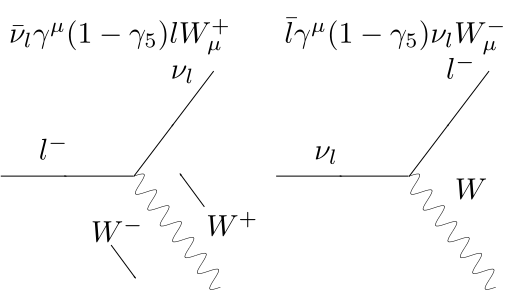
\includegraphics[scale=0.5]{leptoncc}
\qquad  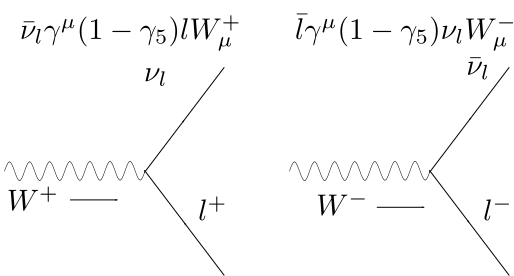
\includegraphics[scale=0.5]{wdecay}

  \caption{Diagramas de Feynman para las corrientes cargadas}
  \label{fig:leptoncc}
\end{figure}
Del primer y cuarto diagrama obtenemos el diagrama de Feynman para el decaimiento $\mu^-\to \nu_\mu e^-\bar{\nu}_e$, mostrado en la figura~\ref{fig:muondecay}
\begin{figure}
  \centering
  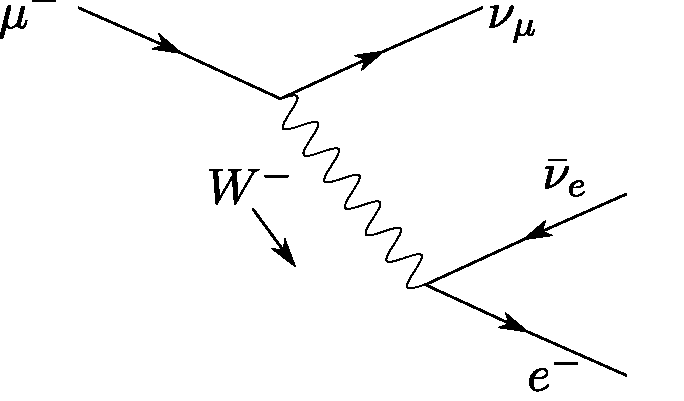
\includegraphics[scale=0.5]{muon_decay}
  \caption{diagrama de Feynman para el decaimiento $\mu^-\to \nu_\mu e^-\bar{\nu}_e$}
  \label{fig:muondecay}
\end{figure}
El propagador para el bos\'on $W$ de momentum $q$ resulta ser
\begin{align}
  \widetilde{D}_{\mu\nu}=\frac{1}{q^2-m_W^2}\left(g_{\mu\nu}-\frac{q_\mu q_\nu}{m_W^2}\right)\,.
\end{align}
Para los prop\'ositos actuales la obtenci\'on de este resultado no es necesaria, el punto importante es que cuando las masas de las part\'\i culas iniciales y finales son mucho m\'as peque\~nas que $m_W$, esto se reduce a
\begin{align}
  \widetilde{D}_{\mu\nu}=-\frac{g_{\mu\nu}}{m_W^2}\,.
\end{align}
Este resultado se entiende f\'acilmente cuando se compara con el propagador de una part\'\i culas escalar masiva $1/(q^2-M^2)\to-1/M^2$. Las componentes espaciales de $W_\mu$ con $\mu=1,2,3$, a bajas energ\'\i as tienen el mismo propagador que el de una part\'\i cula escalar, mientras $W_0$, tiene el signo opuesto.

El Lagrangiano efectivo para el decaimiento del mu\'on, $\mu^-\to \nu_\mu e^- \bar{\nu}_e$ es entonces
\begin{align}
  \mathcal{L}=&\frac{g^2}{8}\left[\bar{\nu}_\mu\gamma^\mu(1-\gamma_5)\mu\right]\frac{g_{\mu\nu}}{m_W^2}
  \left[\bar{e}\gamma^\nu(1-\gamma_5)\nu_e\right]\nonumber\\
=&\frac{g^2}{8m_W^2}\left[\bar{\nu}_\mu\gamma^\mu(1-\gamma_5)\mu\right]
  \left[\bar{e}\gamma^\nu(1-\gamma_5)\nu_e\right]\nonumber\\
  =&\frac{G_F}{\sqrt{2}}\left[\bar{\nu}_\mu\gamma^\mu(1-\gamma_5)\mu\right]\left[\bar{e}\gamma_\mu(1-\gamma_5)\nu_e\right]\,,
\end{align}
donde
\begin{align}
  \frac{G_F}{\sqrt{2}}=&\frac{g^2}{8m_W^2}\nonumber\\
  =&\frac{g^24}{8g^2v^2}\nonumber\\
  =&\frac{1}{2v^2}\,,
\end{align}
y
\begin{align}
  v=\left(\sqrt{2}G_F\right)^{-1/2}\,.
\end{align}


De otro lado, para el  decaimiento $\beta$, $n\to p e^- \bar{\nu}_e$, de acuerdo a la figura~\ref{fig:neutrondecay}, tenemos

\begin{align}
    \mathcal{L}=\frac{G_\beta}{\sqrt{2}}\left[\bar{p}\gamma^\mu(1-1.26\gamma_5)n\right]\left[\bar{e}\gamma_\mu(1-\gamma_5)\nu_e\right]\,.
\end{align}
\begin{figure}
  \centering
  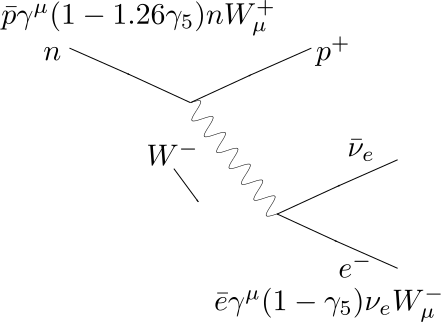
\includegraphics[scale=0.5]{neutrondecay}
  \caption{Decaimiento del neutr\'on.}
  \label{fig:neutrondecay}
\end{figure}
con $G_F$ dado en la ec.~\eqref{eq:233} y $G_\beta=1.10\times10^{-5}\,\text{GeV}^2$. La corriente hadr\'onica tiene la forma V--1.26A. El factor 1.26  puede entenderse como debido a las correcciones a nivel hadr\'onico de una corriente que es de la forma V--A a nivel del quarks, como en la ec.~\eqref{eq:234}. A nivel de quarks el decaimiento del neutr\'on ($udd$) al prot\'on ($uud$) corresponde al decaimiento de uno de los quarks down del neutr\'on $d\to u e^- \bar{\nu}_e$
\begin{align}
    \mathcal{L}=\frac{G_F}{\sqrt{2}}V_{11}\left[\bar{u}\gamma^\mu(1-\gamma_5)d\right]\left[\bar{e}\gamma_\mu(1-\gamma_5)\nu_e\right]\,.
\end{align}
De modo que $G_\beta=G_F V_{11}=G_F\cos\theta_C$, donde $\theta_C$ es el \'angulo de Cabbibo. Una vez se tienen en cuenta correcciones electrod\'ebiles se obtiene el valor $|V_{11}|=0.97418(27)$\cite{PDG}. Las magnitudes de los elementos de la matriz CKM son\cite{PDG}
\begin{align}
  V\approx\begin{pmatrix}
    0.97419&0.2257&0.0359\\
    0.2256&0.97334&0.0415\\
    0.00874&0.0407&0.999133
  \end{pmatrix}\sim \mathbf{1}
\end{align}

\section{C\'alculo de procesos}
\label{sec:calculo-de-procesos}
Se remite al lector al lector a la siguiente parte del curso ``Standard Model and beyond'', de la p\'agina web 

\url{http://gfif.udea.edu.co:2500}

En particular a las secciones iniciales de los Cap\'\i tulos 1 y 2 donde se analizan el decaimiento $W^-\to e^-\bar{\nu}_e$ y el decaimiento del muon. 


\section{Problemas}
\label{sec:problemas-1}
\begin{enumerate}
\item Demuestre expl\'\i citamente la ec.~(\ref{eq:228})
\label{item:chap6.1}
\end{enumerate}


% \left(\right)
%
%%% Local Variables: 
%%% mode: latex
%%% TeX-master: "fullnotes"
%%% End: 
